%tout ce qui est dans ce chapitre doit etre succint%
%l'approfondissement se fera dans la seconde partie avec%
%le cas d'étude%

\chapter{L'intelligence artificelle aujourd'hui}
L'intelligence Artificelle est un domaine faisant partie 
des sciences cognitives dont l'objectif est de mettre au
point des techniques et technologies permettant aux 
machines de simuler l'intelligence humaine ou animale.
Nous pouvons séparer l'IA en deux catégorie distinctes. 

\section{Intelligence Artificielle Faible}
Elle reproduit un comportement de manière le plus précise possible,
en s'ameliorant notamment grâce à l'apprentissage 
mais n'en n'imite pas le fonctionnement ce qui fait que
ce type d'IA ne fait que simuler de l'intelligence. \newline

\begin{figure}[!h]
    \centering
    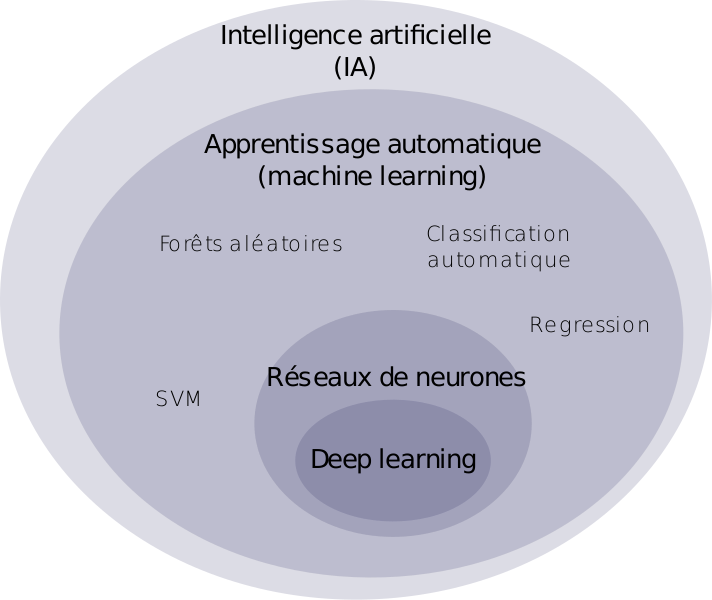
\includegraphics[width=0.8\textwidth]{Images/aitype}
    \caption{Les différents domaines de l'Intelligence Artificielle}
	\label{fig:categorieIA}
\end{figure}


\subsection{Machine Learning}
Le Machine Learning est un ensemble de techniques qui permettent à un ordinateur 
d'agir et d'apprendre d'une manière semblable à l'humain tout en s'améliorant 
au fur et à mesure et ce de manière autonome.


\subsection{Deep Learning}
Le Deep Learning est une sous catégorie du machine learning, 
la différence majeur réside dans le fonctionnement du traitement des 
informations  

\begin{figure}[!h]
    \centering
    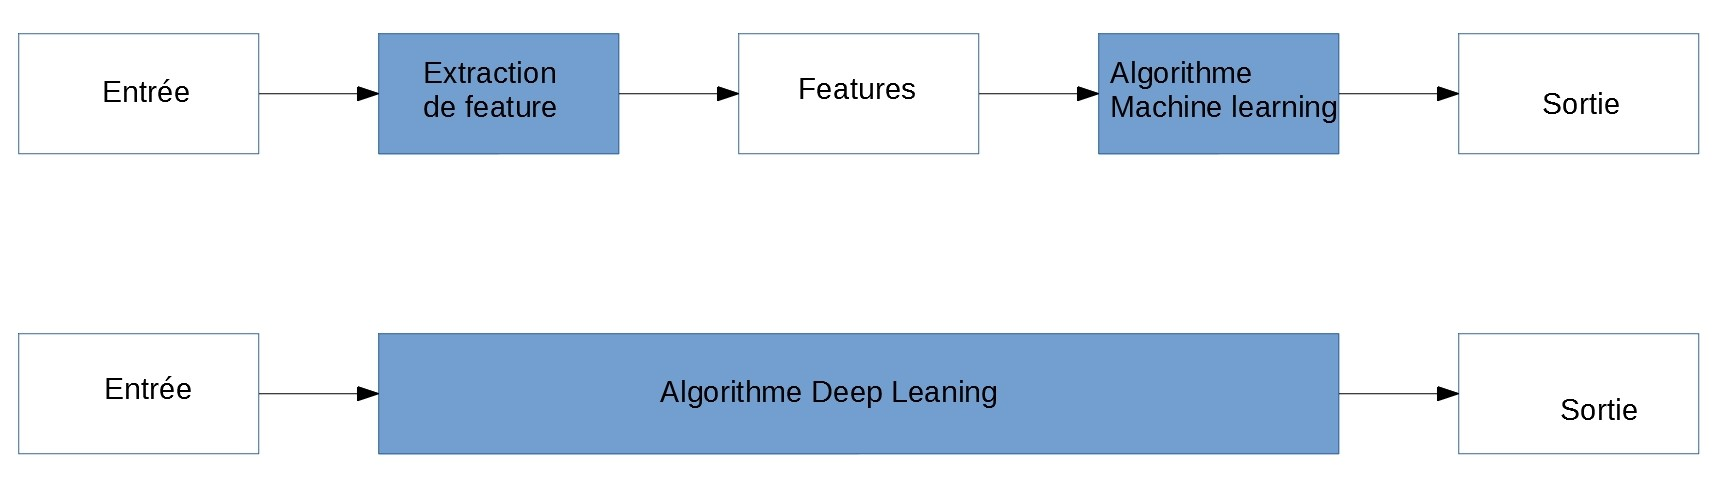
\includegraphics[width=1\textwidth]{Images/MLvsDL}
    \caption{Différences entre machine learning et deep learning}
	\label{fig:categorieIA}
\end{figure}


% à mettre à la fin 
Du point de vue d'un observateur externe, l'IA faible
semble maitriser des concepts mais il n'en n'est rien dans la 
réalité, il suffit de reprendre l'exemple de la reconnaissance d'image
où comme l'IA ne comprend pas les concept et ne peut reconnaitre 
que des éléments correspondant au critères avec lequels elle a été 
entrainé, si on lui présente un élément avec une variance elle 
sera incapable de le reconnaitre.  
    
\section{Intelligence Artificielle Forte}
L'intelligence artificelle forte est l'intelligence
telle qu'elle existe chez l'homme




